\chapter{Construction d'un Générateur de Portefeuilles de Passifs Réaliste}

\section{Objectifs Stratégiques et Contraintes Techniques}
La capacité à tester la robustesse des modèles et la pertinence des analyses de sensibilité repose sur un prérequis fondamental : la disponibilité de données de passif variées et réalistes. Pour un cabinet de conseil, où l'accès aux portefeuilles des clients n'est pas systématique, la faculté de générer des portefeuilles synthétiques, mais représentatifs du marché, constitue un atout stratégique majeur. C'est dans ce contexte qu'un générateur de portefeuilles de passifs a été conçu et développé dans le cadre de ce mémoire.

Ce chapitre a pour vocation de présenter cet outil essentiel. Nous détaillerons les besoins stratégiques et analytiques auxquels il répond, la méthodologie de génération retenue, les contraintes techniques rencontrées et les données qui ont été utilisées pour rendre le portefeuille le plus réaliste possible.

 
\subsection{Définition du générateur de portefeuilles de passifs}
Un générateur de portefeuille de passifs est un outil conçu pour créer, de manière algorithmique, des ensembles de données synthétiques qui imitent avec réalisme des portefeuilles de contrats d'assurance-vie. Plutôt que de s'appuyer sur des données réelles, souvent confidentielles ou indisponibles, cet outil simule les caractéristiques fondamentales des assurés (âge, sexe, etc.) et de leurs contrats (type de produit, montant de la provision mathématique, date de souscription, etc.).

L'objectif n'est pas de produire des données aléatoires, mais de générer un portefeuille dont les propriétés statistiques — distributions, corrélations, tendances — sont indiscernables de celles d'un portefeuille réel. Il s'agit d'une brique essentielle pour l'analyse quantitative en actuariat, permettant de surmonter les contraintes d'accès aux données. Le développement d'un tel outil s'est imposé comme une nécessité pour plusieurs raisons stratégiques et analytiques.


\subsection{Besoins métiers : simulation de nouveaux produits et analyse concurrentielle}
Pour un acteur du secteur de l'assurance, qu'il s'agisse d'un assureur ou d'un cabinet de conseil, la capacité à modéliser et à anticiper les dynamiques de marché est un avantage concurrentiel décisif. Le générateur de portefeuilles de passifs répond directement à ce besoin en fournissant un support quantitatif pour la prise de décision stratégique. Il permet par exemple à un cabinet de conseil de tester ses modèles sans dépendre des données clients, et à un assureur d'explorer des scénarios prospectifs ou d'évaluer l'impact de nouvelles offres. Son utilité se manifeste dans trois domaines clés pour les assureurs : le lancement de nouveaux produits, l'orientation du \textit{business mix} et l'analyse concurrentielle.

Premièrement, le lancement d'un nouveau produit d'assurance-vie représente un investissement et un risque significatifs. Avant toute commercialisation, il est impératif d'en évaluer rigoureusement les impacts sur le profil de risque et la rentabilité de l'entreprise. Le générateur offre un véritable laboratoire virtuel pour effectuer ces tests. En simulant l'intégration de milliers de polices conformes aux caractéristiques du nouveau produit (garanties, frais, options), il permet de projeter leur comportement dans le temps. Il devient alors possible d'analyser leur effet sur les indicateurs prudentiels de Solvabilité II, tels que le \textit{Best Estimate} (BE) et le \textit{Solvency Capital Requirement} (SCR), mais aussi d'évaluer leur sensibilité à divers chocs de marché (hausse des taux, krach boursier) ou de comportement (vagues de rachats). Cet outil permet ainsi de tester, d'ajuster et d'optimiser les caractéristiques d'un produit pour atteindre le couple rendement/risque désiré avant même sa mise sur le marché.

Deuxièmement, le générateur est un outil précieux pour piloter la stratégie à long terme de l'entreprise. La direction peut être amenée à vouloir faire évoluer son \textit{business mix}, c'est-à-dire la répartition de son portefeuille entre différents types de produits (fonds en euros, unités de compte, prévoyance...). Par exemple, dans un contexte de taux bas persistants, un assureur pourrait vouloir accélérer sa transition vers les produits en unités de compte. Le générateur permet de quantifier les implications d'une telle stratégie. En simulant des portefeuilles futurs correspondant à ces nouvelles orientations commerciales, la direction peut visualiser les conséquences sur le bilan, la rentabilité prévisionnelle, mais aussi sur la consommation de capital et l'exposition aux risques. Ces simulations éclairent les décisions stratégiques et s'intègrent naturellement dans des exercices prospectifs comme l'ORSA (\textit{Own Risk and Solvency Assessment}).

Enfin, la capacité à se positionner par rapport à ses concurrents est fondamentale. Faute d'accès aux portefeuilles détaillés des autres acteurs, un assureur doit s'appuyer sur des reconstitutions. En se basant sur des données publiques (rapports annuels ou publications réglementaires comme les SFCR) ou des statistiques sectorielles, le générateur peut permettre la création d'un portefeuille représentatif du marché, ou simuler le portefeuille probable d'un concurrent spécifique. Ces portefeuilles synthétiques deviennent alors une base solide pour des analyses comparatives (\textit{benchmarking}). Ils permettent non seulement d'évaluer la performance relative, mais aussi de comparer les profils de risque, d'anticiper les stratégies concurrentes et d'identifier les meilleures pratiques du marché. Il convient toutefois de souligner les limites d'une telle démarche. Une analyse ALM complète et réaliste d'un concurrent ne peut se contenter de la seule modélisation du passif. Elle exigerait également de simuler son portefeuille d'actifs et de disposer d'informations précises sur ses ressources financières et ses fonds propres. Or, ces données, qui relèvent du secret des affaires, sont rarement publiques. Par conséquent, l'analyse comparative reste nécessairement partielle, se concentrant sur les caractéristiques intrinsèques du portefeuille de passifs reconstitué.
\bigskip

\begin{figure}[h!]
    \centering
    \begin{tikzpicture}[
        node distance=1ex,
        box/.style={
            rectangle,
            rounded corners=4pt,
            draw=gray,
            fill=white,
            very thin,
            inner sep=15pt,
            minimum width=3cm,
            minimum height=2cm,
            align=center,
            font=\sffamily\bfseries\color{black}
        },
        arrow/.style={
            -Latex,
            very thin,
            color=accenture,
            line width=2pt
        }
    ]

    % Nodes
    \node[box] (input) {Données d'entrée :\\- Rapports d'assureurs\\- Marché français};
    \node[box, right=4ex of input] (process) {Modélisation et calibrage :\\- Distributions\\- Corrélations};
    \node[box, right=4ex of process] (output) {Portefeuille synthétique};

    % Arrows
    \draw [arrow] (input) -- (process);
    \draw [arrow] (process) -- (output);

    \end{tikzpicture}
    \caption{Schéma de la méthodologie de génération d'un portefeuille de passifs synthétique.}
    \label{fig:methodologie_horizontale}
\end{figure}

\subsection{Défis de la modélisation : réalisme, volumétrie et flexibilité}

La conception et la mise en œuvre d'un générateur de portefeuilles de passifs efficace soulèvent trois défis majeurs et interdépendants :

\begin{itemize}
\item \textbf{Le réalisme des données générées :} Il s'agit du défi le plus fondamental. L'objectif n'est pas de produire des données aléatoires, mais de créer un portefeuille synthétique dont les propriétés statistiques sont indiscernables de celles d'un portefeuille réel. Cela implique non seulement de reproduire fidèlement les distributions de chaque caractéristique individuelle (âge, montant, etc.), mais aussi, et surtout, de capturer les corrélations complexes qui les lient. Par exemple, l'âge d'un assuré est souvent corrélé au type de produit souscrit et au montant de sa provision mathématique. Ignorer ces dépendances conduirait à un portefeuille incohérent, dont le comportement sous différents scénarios de risque serait erroné, invalidant ainsi les analyses prudentielles ou stratégiques qui en découlent.

\item \textbf{La gestion de la volumétrie :} Les portefeuilles d'assurance-vie des grands acteurs du marché se comptent en centaines de milliers, voire en millions de contrats. Le générateur doit être capable de produire des ensembles de données de cette ampleur de manière performante, c'est-à-dire dans un temps de calcul raisonnable et sans consommer une quantité prohibitive de ressources mémoire. Cette contrainte de performance est d'autant plus forte que la gestion des corrélations, nécessaire au réalisme du portefeuille, ajoute une complexité de calcul significative. Il faut donc trouver un équilibre entre la sophistication statistique et la performance, ce qui a des implications directes sur les choix technologiques et algorithmiques.

\item \textbf{La flexibilité de l'outil :} Un générateur ne serait que d'une utilité limitée s'il ne produisait qu'un seul type de portefeuille statique. Pour répondre aux besoins métiers variés, l'outil doit être hautement paramétrable. L'utilisateur doit pouvoir ajuster finement les caractéristiques du portefeuille à générer : définir les spécificités d'un nouveau produit, modifier les distributions statistiques pour simuler un segment de marché différent, ou encore changer les lois de comportement (rachat, mortalité) pour tester de nouvelles hypothèses. Cette flexibilité est la clé qui transforme le générateur en un véritable laboratoire d'expérimentation pour les actuaires et les stratèges.
\end{itemize}

Relever ces trois défis a nécessité de concevoir une architecture alliant rigueur statistique et performance calculatoire. La section suivante présente en détail la méthodologie de modélisation probabiliste qui a été développée pour construire un portefeuille à la fois réaliste, volumineux et flexible.

\section{Méthodologie de Génération et Modélisation Statistique}

La méthodologie de génération du portefeuille de passifs synthétique repose sur une approche probabiliste. L'objectif est de construire un ensemble de contrats d'assurance dont les propriétés statistiques sont entièrement maîtrisées. Pour ce faire, chaque caractéristique d'un contrat (âge de l'assuré, montant de la provision, etc.) est modélisée comme une variable aléatoire, tirée d'une loi de probabilité préalablement calibrée sur des données de marché quand elles sont disponibles. Sinon, des hypothèses ont été formulées pour recréer ces variables de la manière la plus réaliste possible.


\subsection{Approche stochastique par lois de probabilité}

Le cœur du générateur de passifs repose sur la modélisation de chaque attribut d'un contrat d'assurance vie par une loi de probabilité spécifique. Ce processus permet de créer une population de polices hétérogène et réaliste, dont la diversité est essentielle pour une simulation ALM pertinente. La génération s'effectue en deux temps : d'abord, la définition de "produits types" ou archétypes, puis la génération des contrats individuels à partir de ces archétypes. \textit{Note pour moi-même : Le concept d'archétypes est une bonne idée, mais je dois le rendre plus concret. Je devrais définir précisément ce que c'est, combien j'en ai créé et sur quelle base (ex: "fonds en euros sécuritaire", "mixte dynamique", "pur UC"). Un tableau récapitulatif des archétypes et de leurs caractéristiques serait une excellente addition pour clarifier ce point.}

Les caractéristiques de ces profils (par exemple, les fourchettes de Taux Minimum Garanti (TMG), les montants moyens de provision mathématique) sont elles-mêmes générées aléatoirement à l'aide de lois uniformes, discrètes ou continues. Cette première étape permet de fixer les méta-paramètres (tels que la moyenne $\mu$, l'écart-type $\sigma$, ou les bornes $[min, max]$) qui régiront la génération fine des contrats. \textit{Note pour moi-même : Attention, ce passage est confus. Est-ce que je tire les paramètres des archétypes aléatoirement ? Si c'est le cas, je dois justifier cette couche de stochasticité. Sinon, si les paramètres sont fixés par des hypothèses expertes, je dois le dire clairement. Je devrais reformuler en précisant que "Les paramètres définissant chaque archétype (fourchettes de TMG, etc.) sont déterminés en amont..." pour plus de clarté.}

Chaque contrat individuel est ensuite instancié en tirant ses variables selon des lois de probabilité spécifiques, reflétant la nature de la caractéristique modélisée :
\subsubsection{Exemple de calibration : Modélisation de la distribution des âges}
Une modélisation précise de la distribution de l'âge est essentielle lorsque l'on souhaite modéliser un portefeuille de passifs. En effet, c'est un facteur clé dans l'évaluation de risques tels que le décès. La démarche de modélisation s'est déroulée en quatre étapes principales : la préparation des données, l'ajustement de modèles, la comparaison statistique et la sélection du meilleur modèle.

La première étape a consisté à construire une distribution de probabilité réaliste à partir de deux sources de données :
\begin{enumerate}
\item \textbf{La pyramide des âges de la population française} pour l'année 2024 \cite{pyramide_age}, fournissant la structure démographique de base entre 0 et 100 ans.
\begin{figure}[H]
\centering
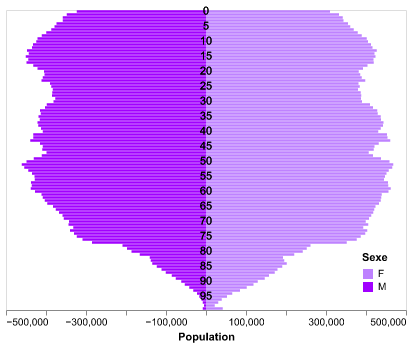
\includegraphics[width=0.9\textwidth]{images/2_chapitres/chapitre3/pyramide_age.png}
\caption{Pyramide des âges de la population française en 2024 \cite{pyramide_age}.}
\label{fig:pyramide_age}
\end{figure}
\item \textbf{Une étude statistique de l'INSEE} sur la détention d'assurance-vie par tranche d'âge en France \cite{insee_prop_av_age}
\begin{figure}[H]
\centering
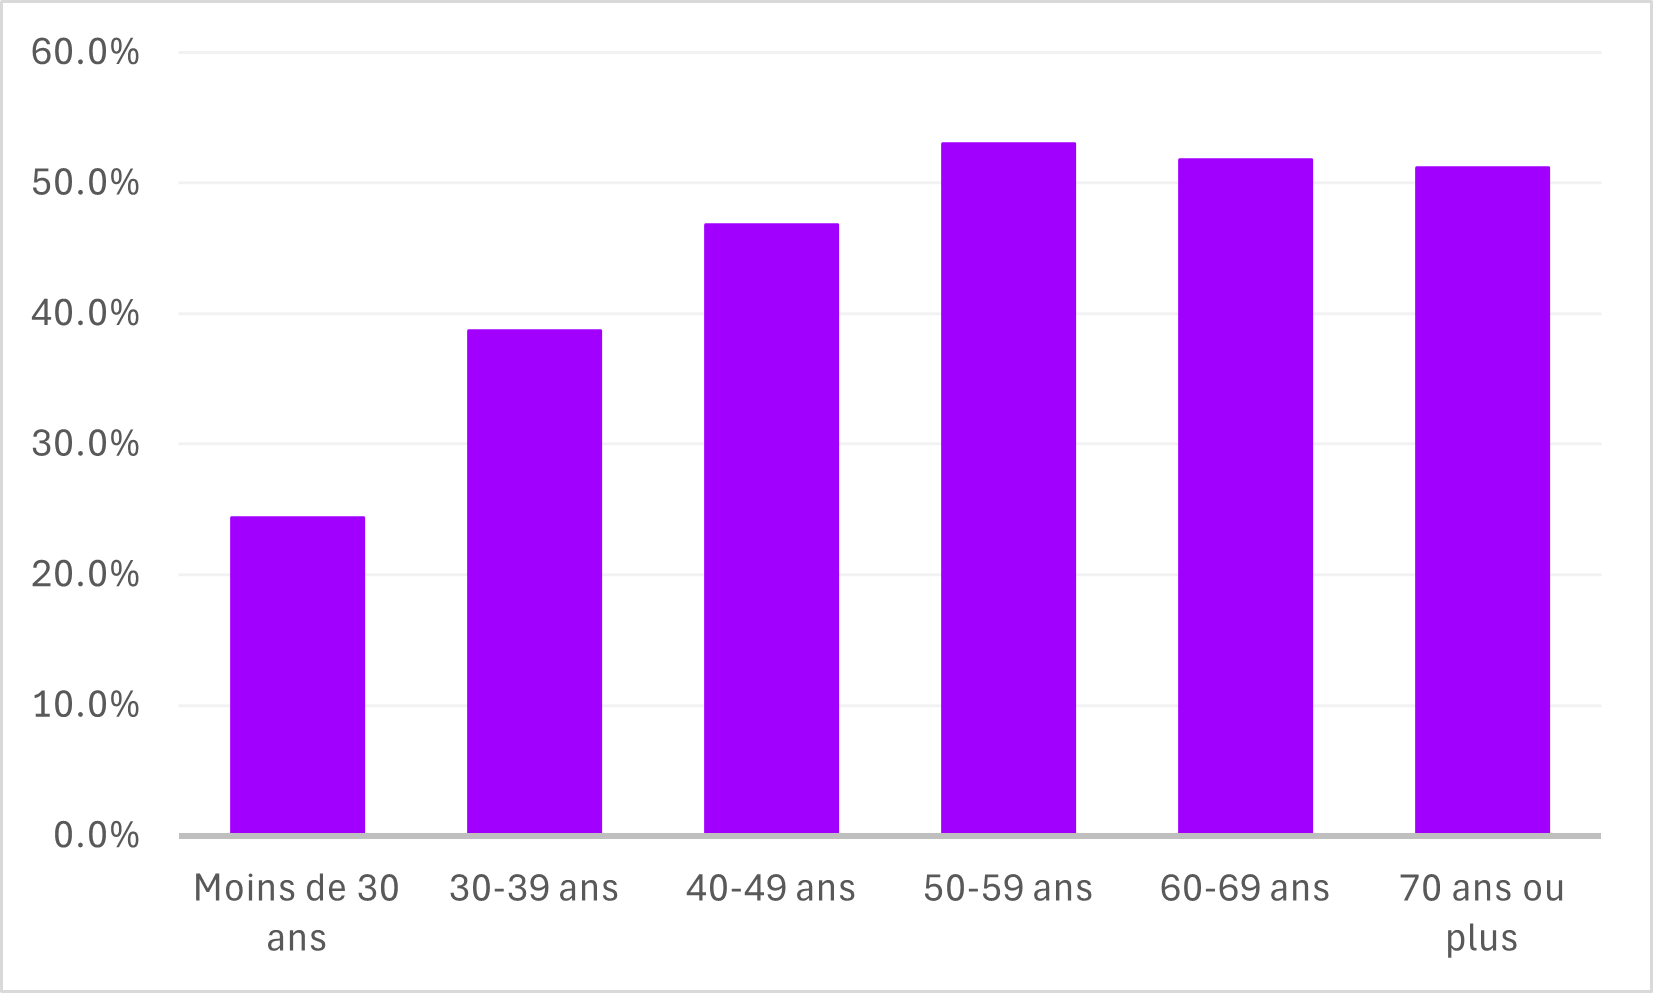
\includegraphics[width=0.7\textwidth]{images/2_chapitres/chapitre3/insee_prop_av_age.png}
\caption{Proportion de détention d'assurance-vie par tranche d'âge en France \cite{insee_prop_av_age}.}
\label{fig:insee_prop_av_age}
\end{figure}
\end{enumerate}

Afin d'obtenir de passer de la figure \ref{fig:insee_prop_av_age} à une proportion de personnes possédant une assurance vie par age, il a été décidé de faire plusieurs interpolations entre les points de données fournis. 
Il a d'abord été décidé de définir des points précis pour chaque tranche d'âge, en prenant la moyenne de chaque tranche. Par exemple, pour la tranche 18-30 ans, le point retenu est 24 ans. Pour la dernière tranche "70 ans et plus", le point retenu est 82.5 ans. Ensuite une interpolation par spline cubique a été réalisée entre les points de 24 ans à 64.5 ans. Pour atteindre le point suivant, 82.5 ans, une interpolation linéaire a été effectuée afin d'obtenir une décroissance réaliste. Puis après 82.5 ans, il a été décidé de garder la proportion constant car on prend en hypothèse que personne ne souscrit ou ne part de l'assurance vie après 82.5 ans.
Ces interpolations permettent d'obtenir une estimation continue du taux de détention pour chaque âge entre 18 et 100 ans, qui est l'âge maximum retenu dans le cadre de la génération de portefeuilles dans le cadre de cette étude. 
\begin{figure}[H]
\centering
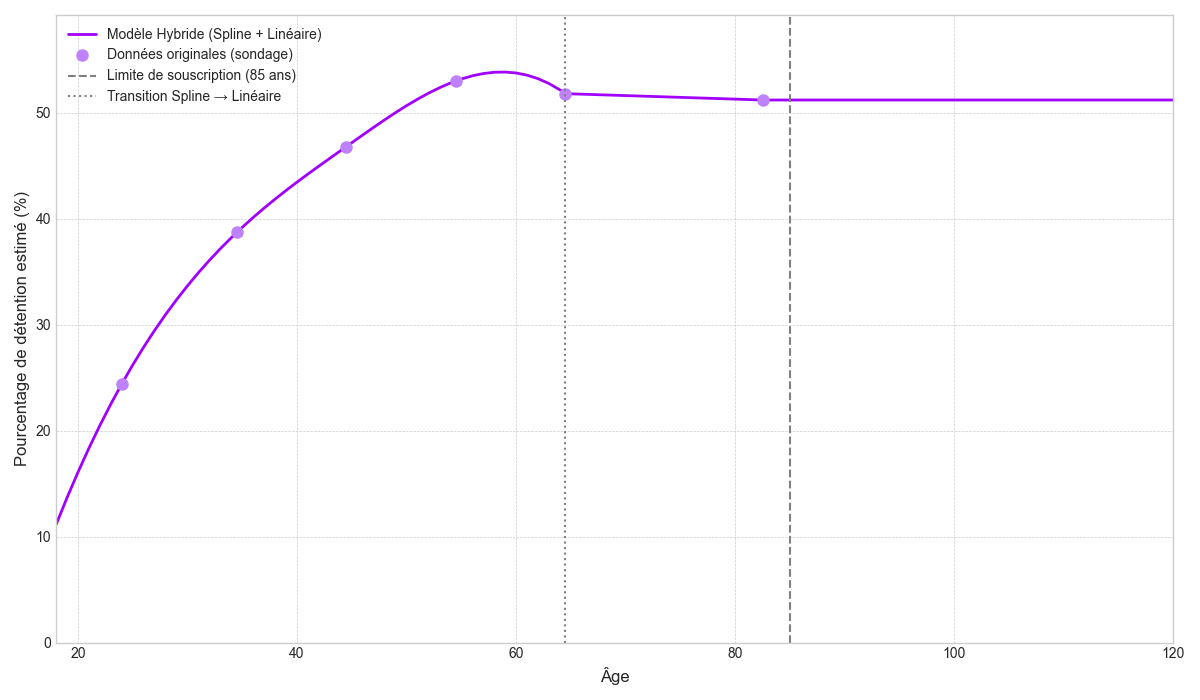
\includegraphics[width=0.7\textwidth]{images/2_chapitres/chapitre3/interpolation_prop_age.png}
\caption{Proportion de détention d'assurance-vie par âge en France par diverses méthodes d'interpolation.}
\label{fig:interpolation_prop_age}
\end{figure}


En multipliant la population de chaque âge par le taux de détention estimé, il a été possible d'obtenir une estimation du nombre d'assurés pour chaque âge et chaque sexe. Après normalisation, il est désormais possible de construire une loi de probabilité empirique, illustrée par la figure \ref{fig:empirique}.

\begin{figure}[H]
\centering
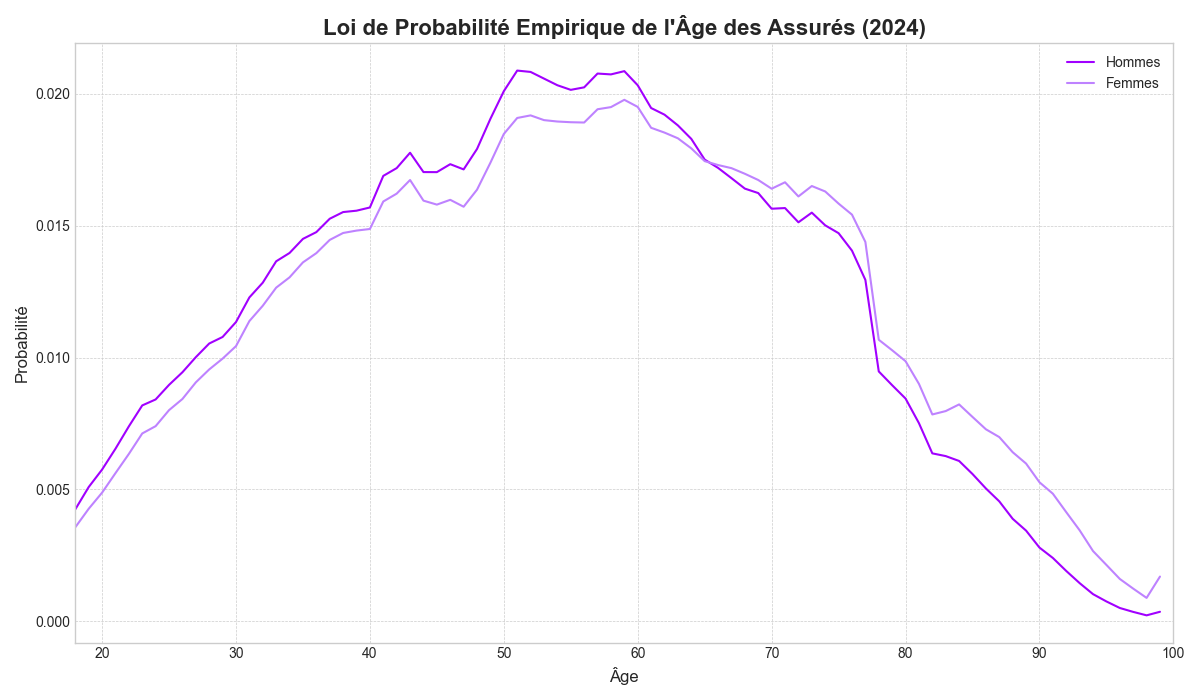
\includegraphics[width=0.9\textwidth]{images/2_chapitres/chapitre3/distribution_age_assures.png}
\caption{Distribution empirique de l'âge des assurés (Hommes et Femmes).}
\label{fig:empirique}
\end{figure}

Deux lois de probabilité continues ont été sélectionnées comme candidates pour modéliser la distribution empirique : la \textbf{loi Gamma} et la \textbf{loi Beta}. Les paramètres de ces deux lois ont été estimés par la méthode du maximum de vraisemblance sur un échantillon de 200 000 individus tirés de la loi empirique. Pour déterminer la loi la plus adéquate, des critères visuels et statistiques (Test de Kolmogorov-Smirnov, AIC, BIC) ont été utilisés. Les figures \ref{fig:gamma} et \ref{fig:beta} montrent l'ajustement des deux lois. Visuellement, la loi Gamma épouse plus fidèlement la forme de la distribution observée.

\begin{figure}[H]
\centering
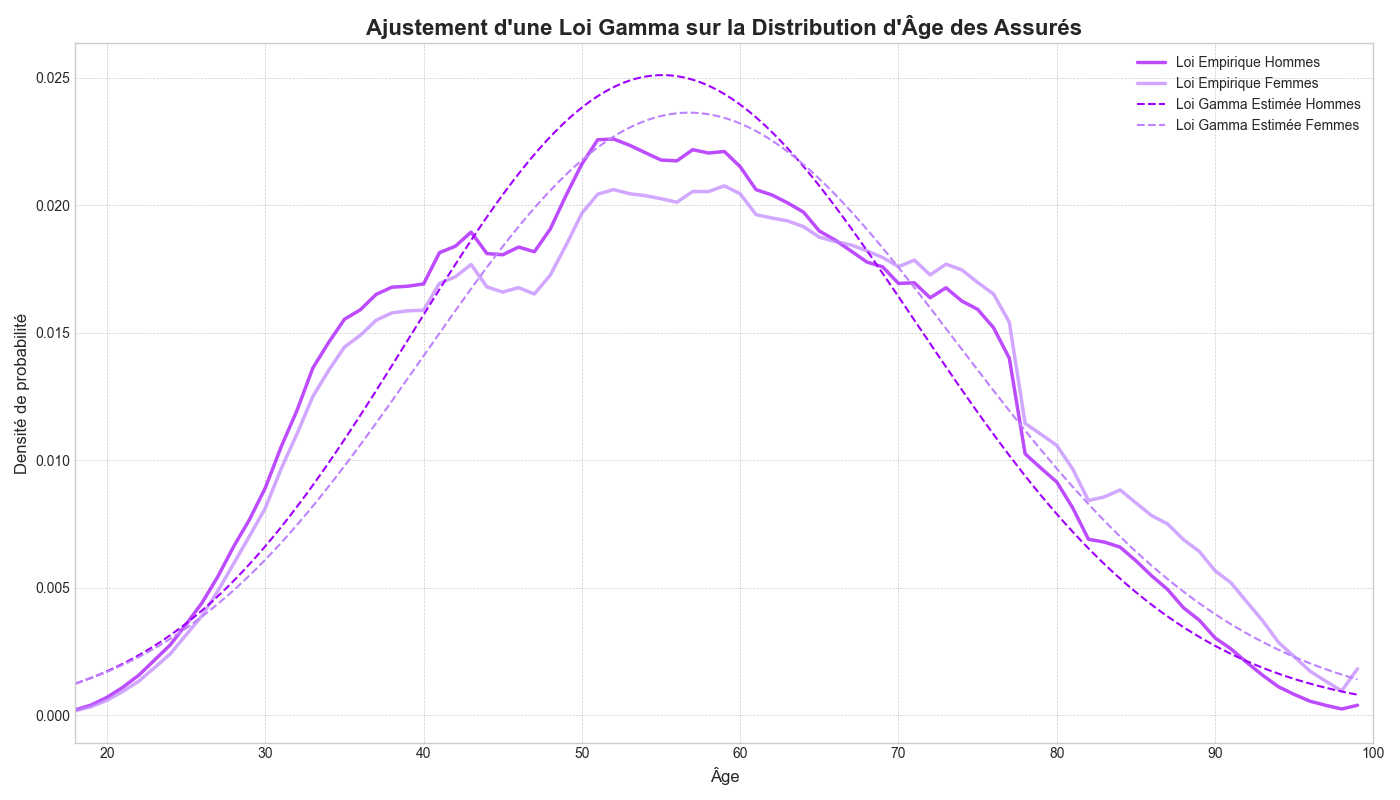
\includegraphics[width=0.9\textwidth]{images/2_chapitres/chapitre3/estimation_loi_gamma.png}
\caption{Ajustement de la loi Gamma sur la distribution empirique.}
\label{fig:gamma}
\end{figure}

\begin{figure}[H]
\centering
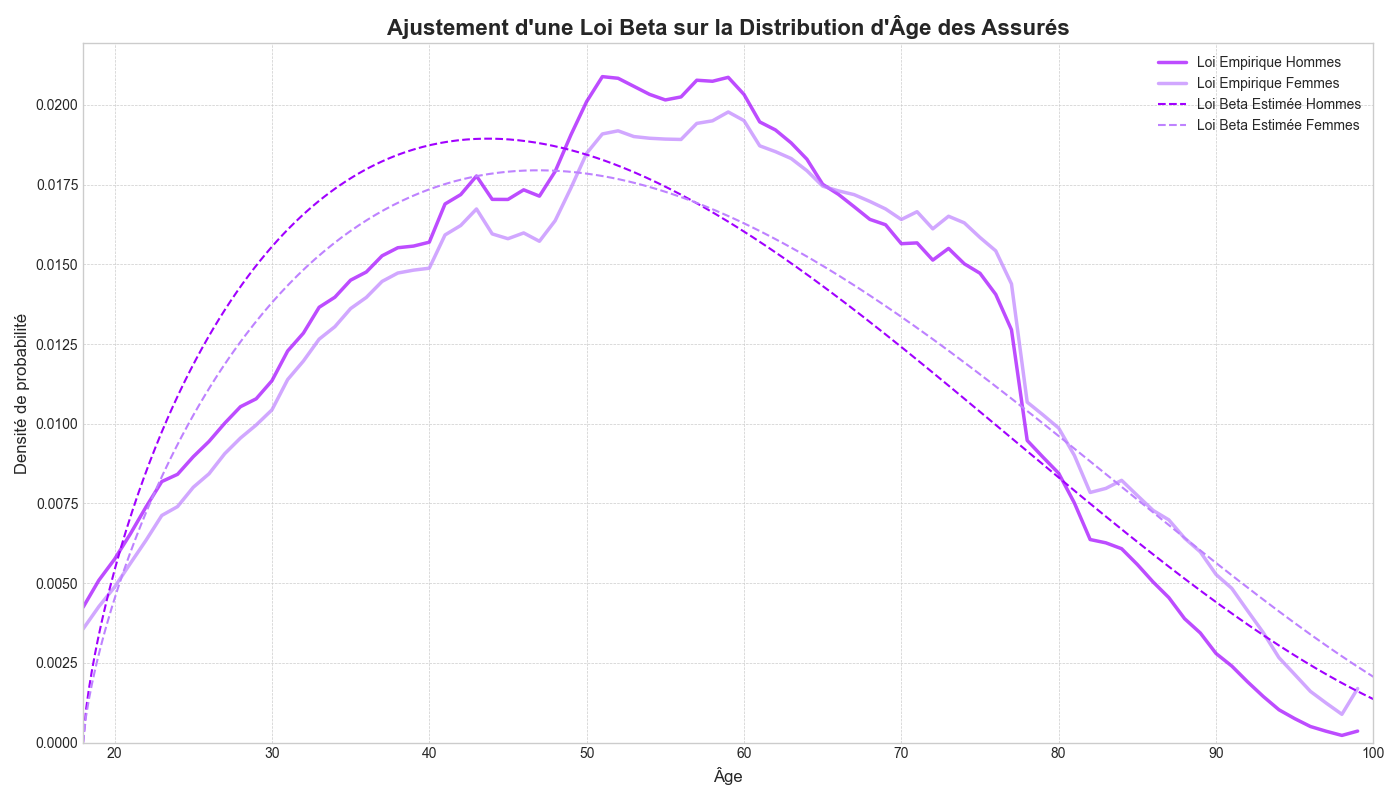
\includegraphics[width=0.9\textwidth]{images/2_chapitres/chapitre3/estimation_loi_beta.png}
\caption{Ajustement de la loi Beta sur la distribution empirique.}
\label{fig:beta}
\end{figure}

Le tableau \ref{tab:stats} confirme cette observation. La loi Gamma présente une statistique K-S deux fois plus faible et des scores AIC et BIC significativement inférieurs, indiquant un meilleur ajustement.

\begin{table}[H]
\centering
\begin{tabular}{@{}lccc@{}}
\toprule
\textbf{Métrique} & \textbf{Loi Gamma} & \textbf{Loi Beta} & \textbf{Meilleur Modèle} \\
\midrule
Statistique K-S (D) & 0.0374 & 0.0748 & Gamma \\
AIC (Akaike) & 1 709 234.40 & 1 718 905.88 & Gamma \\
BIC (Bayésien) & 1 709 265.01 & 1 718 926.30 & Gamma \\
\bottomrule
\end{tabular}
\caption{Tableau comparatif des métriques d'ajustement (population masculine).}
\label{tab:stats}
\end{table}

D'après ces résultats, il est donc recommandé d'utiliser la \textbf{loi Gamma}, avec les paramètres estimés lors de l'analyse, pour toute application nécessitant une génération ou une représentation de l'âge des assurés.



\begin{itemize}
    \item \textbf{Nombre de polices par agrégat :} Modélisé par une loi de Poisson $\mathcal{P}(\lambda)$, tronquée pour assurer une valeur minimale de 1. \textit{Note pour moi-même : Je dois justifier le choix de la loi de Poisson. C'est un choix classique, mais je dois expliquer pourquoi je l'ai fait (ex: grand nombre de clients potentiels, faible probabilité de souscription). Je dois aussi préciser comment le paramètre lambda est calibré. Pour la "troncature à 1", je dois être plus précis mathématiquement. Est-ce que j'utilise une loi de Poisson tronquée en zéro (Zero-Truncated Poisson) ? Si oui, je devrais donner la fonction de masse correspondante.}
    \item \textbf{Sexe de l'assuré :} Modélisé par une loi de Bernoulli $\mathcal{B}(p)$, où $p$ représente la proportion d'hommes définie dans les spécifications du produit. \textit{Note pour moi-même : C'est un choix standard. Je dois juste préciser d'où vient le paramètre p. Est-ce que je l'ai tiré des données de marché, des statistiques nationales (INSEE), ou est-ce une hypothèse propre au produit cible ?}
    \item \textbf{Montants des provisions (fonds euros et UC) :} Tirés selon une loi Normale $\mathcal{N}(\mu, \sigma^2)$, dont les paramètres sont issus des spécifications. Les valeurs générées sont ensuite tronquées pour rester dans des bornes prédéfinies, afin d'éviter les valeurs aberrantes. \textit{Note pour moi-même : Le choix de la loi Normale pour des montants est discutable. Une loi Lognormale ou Gamma serait peut-être plus adaptée. Je dois justifier ce choix. Ai-je fait des tests d'ajustement (Kolmogorov-Smirnov, etc.) sur des données réelles ? Je dois aussi détailler la troncature : quelles bornes [min,max] et comment ont-elles été choisies ? Je dois vérifier si j'ai bien tenu compte de l'impact de la troncature sur la moyenne et la variance pour que les moments finaux correspondent aux cibles.}
    \item \textbf{Allocation d'actifs cible :} Les poids cibles pour chaque classe d'actifs (actions, immobilier, etc.) sont également générés suivant des lois Normales. Un mécanisme de normalisation est ensuite appliqué pour garantir que la somme des allocations $\sum_{i} \omega_i$ pour un contrat donné est égale à 1. \textit{Note pour moi-même : Même remarque que pour les provisions. La normalisation post-tirage modifie les lois marginales. Une approche plus rigoureuse serait d'utiliser une loi de Dirichlet. Je devrais mentionner cette alternative et justifier pourquoi je ne l'ai pas utilisée (par exemple, pour des raisons de simplicité).}
    \item \textbf{Date d'effet du contrat :} Générée par une loi Uniforme continue sur un intervalle de temps $[T_{\text{début}}, T_{\text{fin}}]$. \textit{Note pour moi-même : C'est un choix simple. Je dois le justifier brièvement. Est-ce que l'hypothèse d'une souscription uniforme dans le temps est réaliste pour mon cas ? Je pourrais mentionner que d'autres lois comme Beta ou Triangulaire pourraient mieux modéliser des pics de souscription.}
\end{itemize}

\subsection{Calibration des distributions marginales à partir des données de marché}

L'approche stochastique adoptée n'est pas purement aléatoire ; elle est rigoureusement calibrée pour refléter une réalité de marché ou un portefeuille cible. La calibration des distributions marginales de chaque variable est assurée principalement via un ensemble de spécifications qui définissent les paramètres des lois de probabilité. Ces spécifications peuvent être obtenues de deux manières complémentaires :
\begin{enumerate}
    \item \textbf{Calibration par hypothèses expertes :} Les paramètres des lois (moyennes, écarts-types, bornes) sont définis sur la base d'hypothèses actuarielles et économiques. Cette méthode est utilisée pour explorer des scénarios de marché spécifiques ou pour concevoir des produits cibles. \textit{Note pour moi-même : Ce paragraphe est trop vague, il faut que je le rende plus concret avec des exemples précis.}
    \item \textbf{Calibration directe sur données réelles :} Les spécifications peuvent être issues d'une analyse statistique d'un portefeuille existant. Les paramètres des lois sont alors les estimateurs directs des moments empiriques (moyenne, variance) observés sur les données, garantissant que le portefeuille synthétique réplique fidèlement la structure du portefeuille réel. \textit{Note pour moi-même : C'est le point le plus faible de la section, je dois absolument le renforcer. Je dois décrire précisément la source de données utilisée (portefeuille réel anonymisé ? taille ? période ?). Je dois expliquer la méthode d'estimation (méthode des moments ou maximum de vraisemblance ? Pourquoi ce choix ?). Surtout, je dois ajouter la validation statistique : quels tests d'ajustement (goodness-of-fit) ai-je utilisés (Chi-deux, K-S) et quels sont les résultats (p-valeurs) ? Des graphiques comparant l'histogramme des données réelles et la densité de la loi calibrée sont indispensables ici.}
\end{enumerate}

Un exemple particulièrement abouti de cette calibration est la modélisation de la distribution des âges des assurés. Le processus charge une distribution d'âge de référence, représentative de la population cible. Cette distribution est ensuite transformée en une série de lois de probabilité conditionnelles : pour chaque âge maximum possible à la souscription, $n$, une distribution de probabilité discrète, tronquée à $n$, est calculée. \textit{Note pour moi-même : C'est un bon exemple, mais je dois être plus précis. Quelle est la "distribution d'âge de référence" ? Table de mortalité réglementaire, données INSEE ? Je dois citer la source exacte. Je devrais aussi décrire le processus mathématiquement. Si $f(x)$ est la densité de référence, la densité conditionnelle est $f_{X \mid X \leq n}(x) = \frac{f(x)}{\int_0^n f(t)dt}$. Montrer cette formule prouverait ma maîtrise du sujet.}
Lors de la génération, l'âge d'un assuré pour un contrat donné est tiré au hasard en utilisant la distribution de probabilité conditionnelle qui respecte l'âge maximum autorisé pour ce produit. Cette méthode garantit que la structure démographique du portefeuille généré est cohérente avec celle de la population de référence.

\subsection{Perspective : modélisation des dépendances par la théorie des copules}

\textit{Note pour moi-même : Cette partie devrait plutôt aller dans une conclusion pour donner une ouverture à mon sujet de mémoire}
Une limite inhérente au modèle actuel est l'hypothèse d'indépendance entre les différentes caractéristiques des contrats. Par exemple, le montant de la provision mathématique est généré indépendamment de l'âge de l'assuré, ce qui est une simplification forte de la réalité. Pour dépasser cette limite, une évolution naturelle du modèle consisterait à intégrer la théorie des copules pour modéliser la structure de dépendance entre les variables aléatoires.

La force de l'approche par copules réside dans sa capacité, via le théorème de Sklar, à séparer la modélisation des distributions marginales de celle de leur structure de dépendance. Il serait ainsi possible de conserver la calibration fine de chaque marge, décrite précédemment, tout en introduisant une structure de corrélation réaliste. La mise en œuvre suivrait les étapes suivantes :
\begin{enumerate}
    \item \textbf{Définition de la structure de dépendance :} Spécification d'une matrice de corrélation (par exemple, de Spearman ou de Kendall) entre les variables d'intérêt, comme l'âge, l'ancienneté du contrat et le montant des provisions.\textit{Note pour moi-même : C'est une bonne perspective. Pour la renforcer, je devrais expliquer comment je calibrerais cette matrice de corrélation (estimation à partir des rangs sur les données réelles ?). Je pourrais aussi préciser que le choix entre Spearman et Kendall n'est pas anodin.}
    \item \textbf{Choix d'une famille de copules :} Sélection d'une copule (Gaussienne, de Student, ou archimédienne comme celles de Clayton ou Gumbel) en fonction de la nature des dépendances à modéliser, notamment la symétrie ou la dépendance aux extrêmes (risques de queue).\textit{Note pour moi-même : Parfait. Pour aller plus loin, je pourrais donner un exemple concret : "Par exemple, pour modéliser le fait que les assurés les plus âgés ont tendance à avoir les plus grosses provisions (dépendance dans la queue supérieure), une copule de Gumbel serait plus appropriée qu'une copule Gaussienne." Cela montrerait une compréhension plus fine.}
    \item \textbf{Modification du processus de génération :} Le tirage des variables ne se ferait plus de manière indépendante. Il faudrait d'abord générer des vecteurs de variables uniformes corrélées à partir de la copule choisie. Ensuite, par la méthode de la transformée inverse, appliquer la fonction de répartition inverse de chaque loi marginale calibrée ($F_X^{-1}(u)$) pour obtenir les réalisations des variables finales. \textit{Note pour moi-même : Je dois réfléchir à la faisabilité d'appliquer réellement cette méthode dans le cadre du mémoire.}
\end{enumerate}

Cette extension permettrait d'enrichir considérablement le réalisme du portefeuille synthétique, en capturant des phénomènes clés tels que la tendance des assurés plus âgés à détenir des contrats avec des provisions plus élevées, améliorant ainsi la pertinence des simulations ALM subséquentes.
\section{Présentation de l'Outil et du Portefeuille de Référence Généré}
\subsection{Architecture de l'application en Python et choix technologiques}
% Votre texte ici...
\subsection{Description des paramètres d'entrée et des formats de sortie}
% Votre texte ici...
\subsection{Analyse descriptive du portefeuille de référence}
% Votre texte ici...


% \subsection{Description des contraintes techniques rencontrées}

% La conception du générateur a soulevé plusieurs contraintes techniques. La première fut de garantir le réalisme des portefeuilles générés. Il ne s'agit pas simplement de créer des données aléatoires, mais de reproduire les corrélations observées dans la réalité (par exemple, entre l'âge de l'assuré et le montant des primes). Une autre contrainte était liée à la volumétrie : l'outil devait être capable de générer des portefeuilles de plusieurs millions de lignes de manière performante. Enfin, la flexibilité était un critère essentiel ; l'outil devait permettre de paramétrer finement les caractéristiques des produits à simuler et les lois de comportement (rachat, mortalité) associées.

% \subsection{Méthodologie de génération des portefeuilles}

% La méthodologie adoptée repose sur une approche stochastique. Pour chaque caractéristique clé d'un contrat (âge de l'assuré, montant de la provision mathématique, type de support, etc.), une loi de probabilité a été définie et calibrée à partir de données de marché. L'outil génère ensuite, ligne par ligne, des assurés virtuels en tirant aléatoirement des valeurs selon ces distributions. Pour modéliser les dépendances entre les variables, des techniques de copules ont été envisagées afin de garantir la cohérence et le réalisme des profils générés. Le résultat est un portefeuille granulaire, au contrat près, qui peut ensuite être agrégé en \textit{model points} pour être utilisé dans le modèle de projection ALM.

% \subsection{Présentation de l'outil développé}

% L'outil final se présente comme une application développée en Python, dotée d'une interface permettant à l'utilisateur de paramétrer la simulation. Les entrées principales sont :
% \begin{itemize}
% \item Les caractéristiques du ou des produits à simuler (type de garantie, chargements, etc.).
% \item Les paramètres des lois statistiques pour chaque variable (âge, sexe, montant, etc.).
% \item La taille du portefeuille souhaité.
% \item Les lois de comportement (tables de mortalité, formules de rachat).
% \end{itemize}
% En sortie, l'outil produit un fichier standardisé contenant le portefeuille de passifs généré, directement exploitable par le modèle ALM.

% \section{Choix technologiques et environnement de développement}

% Le passage de VBA à un écosystème Python n'est pas anodin ; il reflète une orientation stratégique vers des technologies plus modernes, ouvertes et performantes, mieux adaptées aux défis du "Big Data" et des calculs intensifs en actuariat.

% \subsection{Migration vers des technologies modernes}
% L'environnement Excel/VBA, bien que très répandu, montre ses limites face à la complexité et à la volumétrie des modèles ALM modernes. La migration vers Python a permis de s'affranchir des limitations de mémoire et de performance d'Excel, tout en bénéficiant d'un langage structuré favorisant la qualité du code, la modularité et les tests automatisés, ce qui est un gage de maintenabilité et de fiabilité à long terme.

% \subsection{Avantages d'un langage open-source}
% Le choix de Python, un langage \textit{open-source}, présente des avantages considérables. D'un point de vue financier, il élimine les coûts de licence associés à de nombreux logiciels propriétaires. Plus important encore, il donne accès à une communauté mondiale de développeurs et de scientifiques, qui contribuent à un écosystème de librairies extrêmement riche et en constante évolution. Cette effervescence garantit un accès permanent aux algorithmes et aux techniques les plus récents.

% \subsection{Utilisation d'un écosystème dynamique}
% Le projet s'est appuyé sur des librairies de pointe pour la manipulation de données et le calcul scientifique. En particulier, l'utilisation de la librairie \textit{Polars} (ou alternativement \textit{Pandas}), écrite en Rust, a permis d'atteindre des niveaux de performance très élevés pour le traitement de grands volumes de données, dépassant de loin les capacités des outils traditionnels. Le fait que ces outils soient mis à jour très fréquemment par la communauté garantit que le modèle bénéficie en permanence des dernières optimisations et fonctionnalités.
